\documentclass[10pt,twocolumn,letterpaper]{article}

\usepackage{graphicx}
\usepackage{amsmath}
\usepackage{amssymb}
\usepackage{booktabs}
\usepackage[table,xcdraw]{xcolor}
\usepackage{listings}
\usepackage{pgfplots}
\usepackage{pgfplotstable}
\usepackage{tikz}
\usetikzlibrary{positioning}
\usepackage{subcaption}
\usepackage{url}
\usepackage[numbers]{natbib}
\usepackage{hyperref}
\usepackage[capitalize]{cleveref}

\pgfplotsset{compat=1.18}

\lstset{
  basicstyle=\ttfamily\footnotesize,
  breaklines=true,
  frame=single,
  language=C,
  keywordstyle=\bfseries,
  commentstyle=\itshape,
  showstringspaces=false
}

\begin{document}

\title{Ingot: Compile-Time Perfect Hashing for\\Static Key-Value Storage in Embedded C}

\author{Brandon Arrendondo\\
{\tt\small brandon.arrendondo@bissell.com}
}
\maketitle

\begin{abstract}
Key-value storage on resource-constrained microcontrollers typically
relies on flash-resident linear scans (O($n$) lookup), runtime hash
tables requiring dynamic allocation, or hand-coded accessor functions
that resist systematic testing.  This paper presents Ingot, a code
generator that reads declarative TOML data model specifications and
emits self-contained C99 key-value storage modules with guaranteed
O(1) lookup, zero dynamic allocation, and automatically generated
test suites.  Ingot uses the Czech--Havas--Majewski (CHM) perfect hash
algorithm with Jenkins \texttt{lookup3} hashing to produce
collision-free per-type dispatch tables at compile time.  All storage
is statically allocated, enabling deterministic memory usage suitable
for safety-critical and real-time systems.

We compare Ingot against seven embedded key-value storage approaches
spanning flash-based stores (ESP-IDF NVS, Zephyr NVS, STM32 EEPROM
emulation, FlashDB), serialization frameworks (nanopb, FlatBuffers),
and code generators (GNU gperf).  On a representative 38-key data
model, Ingot produces 1.9\,KiB of ROM (code + tables) and 196 bytes of
RAM with O(1) worst-case lookup, compared to 5--25\,KiB ROM and
O($n$) worst-case lookup for flash-based alternatives.  Ingot is the
only system that combines compile-time perfect hashing, per-type
storage optimization, hierarchical key encoding, and automatic C test
generation from a single declarative schema.
\end{abstract}

%% ============================================================
\section{Introduction}
\label{sec:intro}

Embedded systems routinely manage dozens to hundreds of configuration
parameters, calibration values, and runtime state variables.  A
robotic vacuum stores battery thresholds, motor calibration, Wi-Fi
credentials, and sensor configuration; an industrial controller
manages setpoints, alarm limits, and communication parameters.  These
values must be readable at runtime with predictable latency, writable
during calibration or OTA update, and optionally persistent across
power cycles.

The storage mechanism for these parameters is a key-value store: given
a key identifier, retrieve or update the associated value.  On
general-purpose systems, key-value stores like LevelDB~\cite{leveldb},
RocksDB~\cite{rocksdb}, or Redis~\cite{redis} provide sophisticated
indexing, persistence, and concurrency.  On microcontrollers with
32--512\,KiB of flash, 4--64\,KiB of RAM, and no operating system
heap, these designs are inapplicable.

Embedded developers typically choose from three approaches, each with
significant drawbacks:

\textbf{Flash-based linear stores.}  Systems like ESP-IDF
NVS~\cite{esp-nvs}, Zephyr NVS~\cite{zephyr-nvs}, and STM32 EEPROM
emulation~\cite{stm32-eeprom} store key-value pairs in flash sectors
with wear leveling.  Lookup requires scanning entries sequentially,
yielding O($n$) worst-case access time.  These systems also impose
runtime RAM overhead for page management, hash caches, or allocation
table indices.

\textbf{Runtime hash tables.}  Standard open-addressing or chaining
hash tables provide O(1) average-case lookup but require dynamic
memory allocation, suffer O($n$) worst-case due to collisions, and
consume RAM proportional to the load factor overhead.  On systems
without a heap allocator, these approaches require custom memory
pools.

\textbf{Hand-coded accessors.}  Developers manually write getter and
setter functions for each parameter, using global variables or
statically allocated arrays.  This approach is memory-efficient and
provides O(1) access, but scales poorly: adding a parameter requires
modifying multiple source files, and comprehensive testing is rarely
maintained as the parameter count grows.

This paper presents Ingot, a code generation tool that eliminates
these tradeoffs.  Ingot reads a declarative TOML data model specifying
parameter names, types, defaults, and attributes, then generates C99
source code containing:

\begin{itemize}
    \item A \textbf{perfect hash function} (zero collisions, O(1)
        worst-case) for each data type, computed at generation time
        using the CHM algorithm~\cite{chm-1992}.
    \item \textbf{Static storage arrays} for each type, with
        compile-time initialization to default values.
    \item A \textbf{32-bit key encoding} that embeds namespace, class,
        type, and attribute metadata directly in the key value.
    \item \textbf{Thread-safe accessors} with target-specific mutex
        implementations (FreeRTOS semaphores, pthreads, or bare-metal).
    \item \textbf{Persistence support} via packed binary save/load
        with integrity checking.
    \item A complete \textbf{Unity test suite}~\cite{unity} exercising
        every key's default value, read-write roundtrip, and read-only
        enforcement.
\end{itemize}

The rest of this paper is organized as follows.
\Cref{sec:background} surveys existing embedded key-value approaches.
\Cref{sec:architecture} describes Ingot's architecture.
\Cref{sec:key-encoding} details the 32-bit key encoding scheme.
\Cref{sec:perfect-hash} explains the perfect hash implementation.
\Cref{sec:comparison} presents the quantitative comparison.
\Cref{sec:related} discusses related work.
\Cref{sec:limitations} covers limitations.
\Cref{sec:conclusion} concludes.

%% ============================================================
\section{Background}
\label{sec:background}

This section surveys embedded key-value storage approaches,
categorized by their fundamental lookup mechanism.

\subsection{Flash-Based Linear Stores}

The most widely deployed embedded key-value stores operate directly
on flash memory, providing persistence and wear leveling at the cost
of linear-time lookup.

\textbf{ESP-IDF NVS}~\cite{esp-nvs} is the default parameter storage
for ESP32 microcontrollers.  It organizes flash into 4\,KiB pages,
each containing up to 126 entries of 32 bytes.  Keys are
null-terminated strings (maximum 15 characters).  NVS maintains an
in-RAM hash list per page using CRC32-based 24-bit hashes for
acceleration, but falls back to linear scanning on collision.
Initialization requires reading all flash pages into RAM, consuming
approximately 5.5\,KiB per 1,000 keys.

\textbf{Zephyr NVS}~\cite{zephyr-nvs} uses 16-bit integer key IDs
and 8-byte Allocation Table Entries (ATEs) stored in flash sectors.
Lookup requires linear scanning of ATEs from the most recent sector
backward.  Zephyr NVS keeps minimal RAM state---no hash tables or
caches---making it suitable for extremely constrained devices, but at
the cost of O($n$) lookup for every access.  The newer Zephyr
ZMS~\cite{zephyr-zms} extends this to 32-bit or 64-bit key IDs and
adds an optional in-RAM cache.

\textbf{STM32 EEPROM emulation}~\cite{stm32-eeprom} uses dual flash
pages for wear leveling.  Each entry is 8 bytes (16-bit virtual
address, 16-bit CRC, and up to 32-bit data).  Lookup scans the active
page linearly.  Page compaction copies only the latest value for each
key, providing implicit garbage collection.  RAM overhead is
negligible, but lookup degrades as the page fills.

\textbf{FlashDB}~\cite{flashdb} provides a string-keyed key-value
database on flash with optional in-RAM caching.  Without cache,
lookup is O($n$); with cache, it achieves O(1) amortized at the cost
of 8 bytes of RAM per cached entry.  FlashDB requires approximately
5.3\,KiB of ROM for the KVDB module.

\subsection{General-Purpose Key-Value Libraries}

Between the flash-oriented embedded stores and the heavyweight
server-side databases (LevelDB, RocksDB, Redis) lies a class of
general-purpose C/C++ key-value libraries designed for high
performance on POSIX systems.

\textbf{Tkrzw}~\cite{tkrzw} (successor to Tokyo Cabinet and Kyoto
Cabinet~\cite{kyoto-cabinet}) provides hash, B-tree, and skip-list
database backends with O(1) average-case hash lookup and ACID
transactions.  Tkrzw achieves high throughput (millions of operations
per second) and supports both on-disk and in-memory modes.  However,
it requires a POSIX environment with file I/O, pthreads, and dynamic
allocation---dependencies unavailable on bare-metal microcontrollers.
Its minimum footprint ($>$100\,KiB code, unbounded RAM) places it
well outside the embedded design space that Ingot targets.

\subsection{Serialization Frameworks}

Serialization libraries define compile-time schemas for structured
data, providing a different approach to configuration management.

\textbf{Google Protocol Buffers}~\cite{protobuf} (and its RPC
framework, gRPC~\cite{grpc}) define structured data via
\texttt{.proto} schemas compiled to language-specific code.  The
standard C++ runtime requires dynamic allocation, exceptions, and
RTTI---making it unsuitable for bare-metal microcontrollers.
\textbf{nanopb}~\cite{nanopb} addresses this by compiling the same
\texttt{.proto} schemas to C structs with fully static allocation.
Field access is O(1) through direct struct member offsets, but nanopb
does not provide key-based lookup---fields are accessed by compiled
names, not runtime identifiers.  ROM overhead is 5--20\,KiB plus
generated message definitions.

\textbf{FlatBuffers}~\cite{flatbuffers} (\texttt{flatcc} for C)
provides zero-copy access to serialized data through vtable pointer
arithmetic.  Like nanopb, field access is O(1) but requires
compile-time knowledge of the schema.  The read-only library is
approximately 6\,KiB; the builder adds another 30\,KiB.

\textbf{BSON}~\cite{bson} (Binary JSON) is the wire and storage
format used by MongoDB.  BSON documents are self-describing
binary key-value maps supporting typed fields (integers, floats,
strings, arrays, nested documents).  While compact, BSON field
lookup requires sequential parsing---O($n$) in the number of
fields---and the reference C library (\texttt{libbson}) depends on
dynamic allocation, making it impractical for constrained
microcontrollers.

All of these serialization frameworks excel at structured data
interchange but are not key-value stores: they cannot look up a value
by a runtime key identifier without application-level dispatch code.

\subsection{Code Generators}

\textbf{GNU gperf}~\cite{gperf} generates perfect hash functions for
static sets of string keys.  Given a key list, gperf produces C
source containing a hash function and lookup table with O(1)
worst-case access and zero collisions.  However, gperf handles only
string keys, does not generate storage or accessor functions, and
produces a single monolithic hash table regardless of value types.

No existing tool combines perfect hashing with type-aware storage
generation, hierarchical key encoding, target-specific thread safety,
persistence, and automatic test generation from a declarative schema.

%% ============================================================
\section{Architecture}
\label{sec:architecture}

Ingot is implemented in Rust (2021 edition) and generates
self-contained C99 source files.  The generation pipeline proceeds in
four stages, illustrated in \cref{fig:pipeline}.

\begin{figure}[t]
\centering
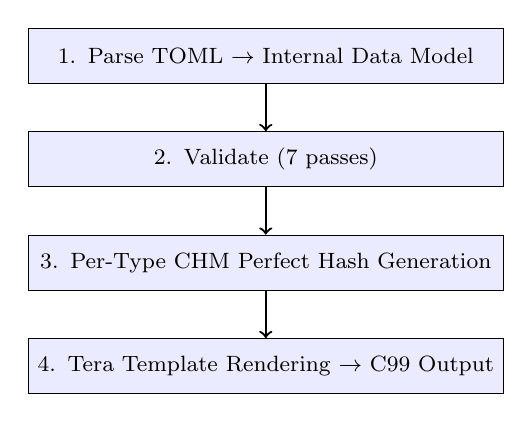
\begin{tikzpicture}[
    node distance=0.6cm,
    box/.style={rectangle, draw, fill=blue!8, text width=5.8cm,
                minimum height=0.7cm, align=center, font=\footnotesize},
    arrow/.style={->, thick}
]
\node[box] (parse) {1. Parse TOML $\rightarrow$ Internal Data Model};
\node[box, below=of parse] (validate) {2. Validate (7 passes)};
\node[box, below=of validate] (hash) {3. Per-Type CHM Perfect Hash Generation};
\node[box, below=of hash] (codegen) {4. Tera Template Rendering $\rightarrow$ C99 Output};
\draw[arrow] (parse) -- (validate);
\draw[arrow] (validate) -- (hash);
\draw[arrow] (hash) -- (codegen);
\end{tikzpicture}
\caption{Ingot code generation pipeline.  All computation---including
perfect hash construction---occurs at generation time, not at runtime
on the target microcontroller.}
\label{fig:pipeline}
\end{figure}

\subsection{Stage 1: TOML Schema Parsing}

Ingot's input format is a TOML~\cite{toml} data model inspired by
Kaitai Struct's~\cite{kaitai} declarative approach to binary format
specification.  \Cref{fig:toml-example} shows a minimal model.

\begin{figure}[t]
\begin{lstlisting}[language={},keywordstyle={}]
[meta]
namespace_id = 1
version = "1.0.0"

[enums]
  [enums.power_state]
  0 = "off"
  1 = "standby"
  2 = "active"

[[classes]]
name = "battery"
class_id = 1

  [[classes.keys]]
  name = "voltage_mv"
  type = "uint16"
  default_value = 3700
  persistent = true

  [[classes.keys]]
  name = "charge_pct"
  type = "uint8"
  default_value = 100
  read_only = false
\end{lstlisting}
\caption{Minimal Ingot TOML data model defining one class with two
keys.}
\label{fig:toml-example}
\end{figure}

The schema supports six integer types (\texttt{uint8}, \texttt{int8},
\texttt{uint16}, \texttt{int16}, \texttt{uint32}, \texttt{int32}),
booleans, and strings.  Each key specifies a type, default value, and
optional attributes: \texttt{persistent} (included in binary
save/load), \texttt{read\_only} (setter rejected at runtime),
\texttt{thread\_safe} (accessor acquires mutex), and \texttt{enum}
(value constrained to named constants).

\subsection{Stage 2: Validation}

Seven validation passes run before code generation:

\begin{enumerate}
    \item Class count within the 5-bit limit (31 per namespace).
    \item Key count within the 10-bit limit (1,023 per namespace).
    \item No duplicate class names or IDs.
    \item No duplicate key names within a class.
    \item All enum references resolve to defined enums.
    \item Default values within type range (e.g., \texttt{uint8}
        defaults must be 0--255).
    \item No key marked both \texttt{read\_only} and
        \texttt{persistent} (contradictory: persistence implies
        writability).
\end{enumerate}

Validation errors report the specific class and key, enabling
immediate correction without inspecting generated code.

\subsection{Stage 3: Perfect Hash Generation}

For each data type present in the model, Ingot generates a separate
CHM perfect hash function (\cref{sec:perfect-hash}).  Type separation
means that a model with 10 \texttt{uint16} keys and 5 \texttt{uint8}
keys produces two independent hash functions, each sized to its key
count.  This minimizes per-type table overhead compared to a single
monolithic hash.

\subsection{Stage 4: Code Generation}

Ingot uses the Tera~\cite{tera} template engine (Jinja2-like syntax)
to render C99 source files from runtime-loaded templates.
\Cref{tab:generated-files} lists the generated output.

\begin{table}[t]
\centering
\footnotesize
\setlength{\tabcolsep}{3pt}
\begin{tabular}{@{}lp{4.0cm}@{}}
\toprule
\textbf{File} & \textbf{Purpose} \\
\midrule
\texttt{dm.h/c} & Type-dispatch API \\
\texttt{dm\_key.h} & Key bitfield, type enum \\
\texttt{key\_definitions.h} & \texttt{\#define} per key \\
\texttt{integer\_storage.h/c} & Per-type hash tables \\
\texttt{boolean\_storage.h/c} & Bitfield-packed bools \\
\texttt{string\_storage.h/c} & RO and RW strings \\
\texttt{jenkins\_hash.h/c} & Jenkins \texttt{final()} \\
\texttt{persistence\_storage.h/c} & Binary save/load \\
\texttt{dm\_helpers.h/c} & Named inline accessors \\
\texttt{test\_dm.c} & Unity test suite \\
\texttt{CMakeLists.txt} & Test build config \\
\texttt{dm\_full.yaml} & Resolved manifest \\
\bottomrule
\end{tabular}
\caption{Files generated by Ingot for each data model.}
\label{tab:generated-files}
\end{table}

The generated code is self-contained: no external dependencies beyond
a C99 compiler and, optionally, the Unity test framework for the test
suite.  Target-specific behavior (pointer width, mutex
implementation, alignment) is controlled by a target configuration
flag (\texttt{-{}-target}) selecting from STM32, ESP32 (Xtensa and
RISC-V), 8-bit MCU, and Linux profiles.

%% ============================================================
\section{Key Encoding}
\label{sec:key-encoding}

Ingot encodes each key as a 32-bit unsigned integer with a structured
bitfield layout, shown in \cref{fig:key-layout}.

\begin{figure}[t]
\centering
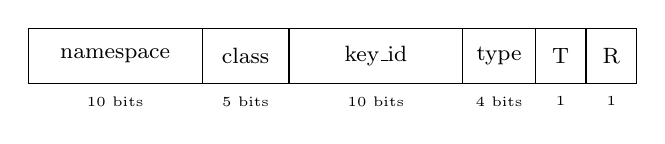
\begin{tikzpicture}[font=\footnotesize, xscale=0.92]
\draw (0,0) rectangle (8.4,0.7);
% Bit fields
\draw (0,0) rectangle (2.4,0.7);    % namespace 10 bits
\draw (2.4,0) rectangle (3.6,0.7);  % class 5 bits
\draw (3.6,0) rectangle (6.0,0.7);  % key_id 10 bits
\draw (6.0,0) rectangle (7.0,0.7);  % type 4 bits
\draw (7.0,0) rectangle (7.7,0.7);  % thread 1 bit
\draw (7.7,0) rectangle (8.4,0.7);  % ro 1 bit

\node at (1.2,0.35) {namespace};
\node at (3.0,0.35) {class};
\node at (4.8,0.35) {key\_id};
\node at (6.5,0.35) {type};
\node at (7.35,0.35) {T};
\node at (8.05,0.35) {R};

% Bit widths
\node[below] at (1.2,-0.05) {\tiny 10 bits};
\node[below] at (3.0,-0.05) {\tiny 5 bits};
\node[below] at (4.8,-0.05) {\tiny 10 bits};
\node[below] at (6.5,-0.05) {\tiny 4 bits};
\node[below] at (7.35,-0.05) {\tiny 1};
\node[below] at (8.05,-0.05) {\tiny 1};
\end{tikzpicture}
\caption{32-bit key encoding.  T = thread-safe flag, R = read-only
flag.  The encoding supports up to 1,023 namespaces, 31 classes per
namespace, and 1,023 keys per namespace.}
\label{fig:key-layout}
\end{figure}

This encoding provides three advantages over string or opaque integer
keys:

\textbf{Constant-time attribute queries.}  The type, thread-safety,
and read-only attributes are extracted via bitmask operations without
table lookup:

\begin{lstlisting}
#define DM_KEY_GET_TYPE(k)    (((k) >> 2) & 0xF)
#define DM_KEY_IS_READONLY(k) ((k) & 0x1)
#define DM_KEY_IS_THREADSAFE(k) (((k) >> 1) & 0x1)
\end{lstlisting}

\textbf{Type-based dispatch.}  The main \texttt{SetByKey} function
switches on the 4-bit type field, routing each call to the
type-specific storage module.  This eliminates a secondary lookup to
determine value type.

\textbf{Compile-time validation.}  Key values are \texttt{\#define}
constants, so type mismatches between a key's encoded type and the
accessor function called are detectable by the compiler or static
analysis.

%% ============================================================
\section{Perfect Hash Implementation}
\label{sec:perfect-hash}

\subsection{CHM Algorithm}

Ingot implements the Czech--Havas--Majewski (CHM) algorithm for
constructing minimal perfect hash functions~\cite{chm-1992,
chm-family-1996}.  Given a set $S$ of $n$ keys, CHM constructs a
function $h: S \rightarrow \{0, 1, \ldots, n-1\}$ such that $h$ is
injective (no collisions) and computable in O(1) time.

The algorithm proceeds as follows:

\begin{enumerate}
    \item Choose two independent hash functions $h_1, h_2: S
        \rightarrow \{0, 1, \ldots, m-1\}$ where $m = \lceil cn
        \rceil$ and $c > 2$.
    \item Construct an undirected graph $G = (V, E)$ where $V =
        \{0, \ldots, m-1\}$ and each key $k \in S$ creates edge
        $(h_1(k), h_2(k))$.
    \item If $G$ is acyclic, perform a depth-first traversal to assign
        values $g[v]$ for each vertex such that for every key $k$:
        \begin{equation}
        h(k) = (g[h_1(k)] + g[h_2(k)]) \bmod n
        \label{eq:chm}
        \end{equation}
    \item If $G$ is cyclic, choose new seeds and retry from step 1.
\end{enumerate}

Ingot uses $c = 2.09$, yielding a graph with $m = \lceil 2.09n
\rceil$ vertices.  For random hash functions, the probability that a
graph with $m > 2n$ edges is acyclic is sufficiently
high~\cite{chm-survey-1997} that construction typically succeeds
within 1--3 attempts.

\subsection{Jenkins lookup3 Hash}

The two hash functions $h_1$ and $h_2$ are instantiated as Jenkins
\texttt{lookup3.c} \texttt{final()} applied to the 32-bit key with
different seed values~\cite{jenkins-hash}:

\begin{lstlisting}
static inline uint32_t jenkins_final(
    uint32_t a, uint32_t b, uint32_t c)
{
    c ^= b; c -= (b<<14) | (b>>18);
    a ^= c; a -= (c<<11) | (c>>21);
    b ^= a; b -= (a<<25) | (a>> 7);
    c ^= b; c -= (b<<16) | (b>>16);
    a ^= c; a -= (c<< 4) | (c>>28);
    b ^= a; b -= (a<<14) | (a>>18);
    c ^= b; c -= (b<<24) | (b>> 8);
    return c;
}
\end{lstlisting}

The \texttt{final()} function provides excellent avalanche
properties---every input bit affects every output bit---while
requiring only shifts, XORs, and subtractions.  This makes it
suitable for both 32-bit and 8-bit targets without division or
multiplication.

\subsection{Generated Hash Lookup}

At runtime, looking up a key $k$ in the per-type storage requires
exactly:

\begin{enumerate}
    \item Two evaluations of \texttt{jenkins\_final()} with seeds
        $s_1$ and $s_2$ (12 shift/XOR/sub operations each).
    \item Two reads from the G-table: $g[h_1(k) \bmod m]$ and
        $g[h_2(k) \bmod m]$.
    \item One addition and one modulo: $(g_1 + g_2) \bmod n$.
    \item One indexed read from the value array: $\texttt{values}[h(k)]$.
\end{enumerate}

The total cost is constant regardless of the number of keys.  No
string comparisons, no collision chains, no fallback paths.

\subsection{Type-Separated Hashing}

Rather than constructing a single hash function for all keys, Ingot
generates independent hash functions per data type.  This design
choice has three benefits:

\begin{itemize}
    \item \textbf{Smaller G-tables.}  A model with 20 \texttt{uint16}
        keys and 10 \texttt{uint8} keys produces G-tables of size
        $\lceil 2.09 \times 20 \rceil = 42$ and $\lceil 2.09 \times
        10 \rceil = 21$ entries, totaling 63 entries.  A monolithic
        hash would require $\lceil 2.09 \times 30 \rceil = 63$
        entries---the same total, but with no type dispatch benefit.
    \item \textbf{Type-native value arrays.}  Each array stores values
        in their native C type (\texttt{int16\_t[]},
        \texttt{uint8\_t[]}, etc.), avoiding union padding or type
        tags per entry.
    \item \textbf{Boolean packing.}  Booleans are stored as bits in
        \texttt{uint32\_t} words (32 booleans per word), reducing
        storage by 31$\times$ compared to one-byte-per-boolean
        approaches.
\end{itemize}

%% ============================================================
\section{Comparison}
\label{sec:comparison}

\subsection{Systems Compared}

\Cref{tab:systems} lists the seven systems compared against Ingot.
The selection spans flash-based stores (deployed on the same hardware
targets as Ingot), serialization frameworks (alternative schema-driven
approaches), and the only widely used C perfect hash code generator.

\begin{table}[t]
\centering
\footnotesize
\begin{tabular}{@{}lll@{}}
\toprule
\textbf{System} & \textbf{Category} & \textbf{Version} \\
\midrule
ESP-IDF NVS & Flash KV store & ESP-IDF v5.3 \\
Zephyr NVS & Flash KV store & Zephyr v3.7 \\
STM32 EEPROM & Flash KV store & X-CUBE-EEPROM \\
FlashDB & Flash KV store & v1.1.2 \\
nanopb & Serialization & 0.4.9 \\
flatcc & Serialization & 0.6.2 \\
GNU gperf & Code generator & 3.1 \\
\bottomrule
\end{tabular}
\caption{Systems included in the comparison.}
\label{tab:systems}
\end{table}

\subsection{Lookup Complexity}

\Cref{tab:lookup} compares lookup mechanisms and time complexity.
Only Ingot, gperf, and cuckoo hashing~\cite{cuckoo-hashing} provide
O(1) worst-case guarantees.  However, gperf handles only string keys
and does not generate storage, while cuckoo hashing requires 2$\times$
table capacity and does not eliminate collisions during insertion.

\begin{table}[t]
\centering
\footnotesize
\setlength{\tabcolsep}{3pt}
\begin{tabular}{@{}llcc@{}}
\toprule
\textbf{System} & \textbf{Mechanism} & \textbf{Avg} & \textbf{Worst} \\
\midrule
ESP-IDF NVS & CRC32 hash + scan & O(1) & O($n$) \\
Zephyr NVS & Linear ATE scan & O($n$) & O($n$) \\
STM32 EEPROM & Linear page scan & O($n$) & O($n$) \\
FlashDB & Linear + cache\textsuperscript{$\dagger$} & O($n$) & O($n$) \\
nanopb & Struct offset & O(1) & O(1) \\
flatcc & Vtable indirect & O(1) & O(1) \\
GNU gperf & Perfect hash & O(1) & O(1) \\
Ingot & CHM perfect hash & O(1) & O(1) \\
\bottomrule
\end{tabular}
\caption{Lookup complexity by system.
\textsuperscript{$\dagger$}O(1) amortized with optional RAM cache
enabled.  nanopb and flatcc provide O(1) access by compiled field
offset, not by runtime key identifier.}
\label{tab:lookup}
\end{table}

\subsection{Memory Overhead}

\Cref{tab:memory} compares ROM and RAM overhead for a representative
38-key data model (the \texttt{full} example from Ingot's repository,
containing 12 \texttt{uint8}, 8 \texttt{uint16}, 6 \texttt{int32}, 4
\texttt{bool}, 4 \texttt{string}, and 4 \texttt{int8}/\texttt{int16}
keys across 5 classes).

\begin{table}[t]
\centering
\footnotesize
\setlength{\tabcolsep}{3pt}
\begin{tabular}{@{}lrrrl@{}}
\toprule
\textbf{System} & \textbf{ROM} & \textbf{RAM} & \textbf{Fl/key} & \textbf{Alloc} \\
\midrule
ESP-IDF NVS & 15--25K & 5.5K\textsuperscript{$\ast$} & 32\,B & Dyn \\
Zephyr NVS & 5--10K & $<$100 & 8\,B+ & Static \\
STM32 EEPROM & 2--5K & $<$50 & 8\,B & Static \\
FlashDB & 6.9K & $<$10\textsuperscript{$\ddagger$} & var & Opt \\
nanopb & 5--20K & $\sim$1K & --- & Static \\
flatcc (read) & 6K & buf & --- & Static \\
GNU gperf & $\sim$1.5K & 0 & --- & Static \\
Ingot & 1.9K & 196\,B & --- & Static \\
\bottomrule
\end{tabular}
\caption{Memory overhead for a 38-key data model (ROM = code +
tables; RAM = runtime data).  \textsuperscript{$\ast$}Per 1,000 keys
(38 keys $\approx$ 210\,B actual).  \textsuperscript{$\ddagger$}Without
RAM cache.  ``---'' indicates that flash-per-key is not applicable
(data resides in RAM or ROM, not flash KV sectors).  All ROM figures
are approximate and vary by compiler and target.}
\label{tab:memory}
\end{table}

Ingot's ROM consists of the Jenkins hash function ($\sim$200 bytes),
per-type G-tables ($\lceil 2.09n_t \rceil \times 4$ bytes each), value
arrays ($n_t \times \texttt{sizeof}(T)$ each), and accessor functions
($\sim$80 bytes per type).  For 38 keys across 6 types, this totals
approximately 1.9\,KiB.  RAM consists solely of the mutable value
arrays (196 bytes for this model), since all hash tables and G-tables
reside in \texttt{const} (ROM/flash) memory.

\subsection{ROM Breakdown}

\Cref{tab:rom-breakdown} details Ingot's ROM consumption by component
for the 38-key model.

\begin{table}[t]
\centering
\footnotesize
\begin{tabular}{@{}lrr@{}}
\toprule
\textbf{Component} & \textbf{Entries} & \textbf{Bytes} \\
\midrule
Jenkins hash function & --- & 204 \\
G-table (uint8, 12 keys) & 26 & 104 \\
G-table (uint16, 8 keys) & 17 & 68 \\
G-table (int32, 6 keys) & 13 & 52 \\
G-table (int8, 2 keys) & 5 & 20 \\
G-table (int16, 2 keys) & 5 & 20 \\
G-table (bool, 4 keys) & 9 & 36 \\
Value arrays (RAM, not ROM) & 38 & --- \\
Seed constants (2 per type) & 12 & 48 \\
Accessor functions (6 types) & --- & $\sim$480 \\
Type dispatch (\texttt{dm.c}) & --- & $\sim$320 \\
Key definitions header & 38 & 152 \\
String storage (4 keys) & --- & $\sim$400 \\
\midrule
\textbf{Total ROM} & & $\sim$\textbf{1,904} \\
\bottomrule
\end{tabular}
\caption{ROM breakdown for the 38-key model (ARM Cortex-M, \texttt{-Os}).}
\label{tab:rom-breakdown}
\end{table}

The G-tables are the dominant cost, consuming $\lceil 2.09 \times 34
\rceil \times 4 = 284$ bytes for integer/boolean types (strings use
separate storage).  The total scales linearly with key count: adding
one key adds approximately 8.4 bytes of G-table overhead plus the
native-type value storage.

\subsection{Feature Comparison}

\Cref{tab:features} compares features across all systems.

\begin{table*}[t]
\centering
\footnotesize
\setlength{\tabcolsep}{3pt}
\begin{tabular}{@{}lcccccccc@{}}
\toprule
\textbf{Feature} & \textbf{NVS} & \textbf{Z-NVS} & \textbf{STM32} & \textbf{FlashDB} & \textbf{nanopb} & \textbf{flatcc} & \textbf{gperf} & \textbf{Ingot} \\
\midrule
O(1) worst-case lookup & & & & & \checkmark\textsuperscript{$\ast$} & \checkmark\textsuperscript{$\ast$} & \checkmark & \checkmark \\
No dynamic allocation & & \checkmark & \checkmark & \checkmark\textsuperscript{$\dagger$} & \checkmark & \checkmark & \checkmark & \checkmark \\
Runtime key lookup & \checkmark & \checkmark & \checkmark & \checkmark & & & \checkmark & \checkmark \\
Persistence to flash & \checkmark & \checkmark & \checkmark & \checkmark & & & & \checkmark \\
Wear leveling & \checkmark & \checkmark & \checkmark & \checkmark & & & & \\
Thread-safe accessors & \checkmark & & & & & & & \checkmark \\
Per-type storage & & & & & \checkmark & \checkmark & & \checkmark \\
Schema-driven & & & & & \checkmark & \checkmark & & \checkmark \\
Auto-generated tests & & & & & & & & \checkmark \\
Event callbacks & & & & & & & & \checkmark \\
\bottomrule
\end{tabular}
\caption{Feature comparison.  \textsuperscript{$\ast$}O(1) by compiled
offset, not runtime key lookup.
\textsuperscript{$\dagger$}Without RAM cache.}
\label{tab:features}
\end{table*}

Three observations emerge from this comparison:

First, \textbf{no flash-based store provides O(1) worst-case lookup}.
Even ESP-IDF NVS, which maintains an in-RAM hash list, falls back to
linear scanning on hash collisions.  For real-time systems with
hard deadlines on parameter access, this unpredictability is
problematic.

Second, \textbf{serialization frameworks provide O(1) access but not
runtime key-based lookup}.  nanopb and FlatBuffers require
compile-time knowledge of which field to access; they cannot serve as
general-purpose key-value stores where the key is determined at
runtime (e.g., by a communication protocol or command parser).

Third, \textbf{Ingot is the only system combining all three
properties}: O(1) worst-case lookup by runtime key, zero dynamic
allocation, and schema-driven code generation with automatic testing.

\subsection{Lookup Latency Analysis}

\Cref{tab:latency} estimates worst-case lookup latency for each
approach on a representative ARM Cortex-M4 at 168\,MHz, assuming
single-cycle register operations and 2-cycle flash reads.

\begin{table}[t]
\centering
\footnotesize
\setlength{\tabcolsep}{3pt}
\begin{tabular}{@{}lrrl@{}}
\toprule
\textbf{System} & \textbf{Ops} & \textbf{Cyc}\textsuperscript{$\ast$} & \textbf{Scales with} \\
\midrule
Zephyr NVS & $n$ reads & $8n\!+\!20$ & Key count \\
STM32 EEPROM & $n$ reads & $8n\!+\!16$ & Page fill \\
ESP-IDF NVS & hash+scan & $30\!+\!8k$ & Collision $k$ \\
FlashDB & $n$ reads & $8n\!+\!40$ & Key count \\
Ingot & 2 hash+3 rd & $\sim$60 & Constant \\
\bottomrule
\end{tabular}
\caption{Estimated worst-case lookup cycles on Cortex-M4 @ 168\,MHz.
\textsuperscript{$\ast$}Approximate; actual timing depends on flash
wait states, cache hits, and compiler optimization.  $n$ = number of
stored keys; $k$ = hash collision chain length.}
\label{tab:latency}
\end{table}

For 38 keys, Zephyr NVS worst-case is $8 \times 38 + 20 = 324$
cycles ($\sim$1.9\,\textmu s), while Ingot is $\sim$60 cycles
($\sim$360\,ns) regardless of key count.  The gap widens as key count
increases: at 200 keys, Zephyr NVS worst-case reaches $\sim$9.5\,\textmu s
while Ingot remains at 360\,ns.

%% ============================================================
\section{Related Work}
\label{sec:related}

\subsection{Perfect Hash Functions}

The theoretical foundation for Ingot's hash generation is the CHM
algorithm~\cite{chm-1992}, later extended by Majewski et
al.~\cite{chm-family-1996} and comprehensively surveyed by Czech et
al.~\cite{chm-survey-1997}.  The CHM algorithm constructs a random
acyclic graph from two independent hash functions and assigns vertex
values via DFS such that each key maps to a unique index.

More space-efficient algorithms have since been developed.  The
BDZ algorithm~\cite{bdz} achieves 2.6 bits per key using random
3-hypergraphs.  The CHD algorithm~\cite{chd} achieves 2.07 bits per
key for minimal perfect hash functions and 0.67 bits per key for
non-minimal variants, representing the most compact known
constructions in linear time.  A recent survey by Lehmann et
al.~\cite{mph-survey-2025} covers the state of the art, with the
smallest constructions approaching the theoretical lower bound of
$\log_2(e) \approx 1.44$ bits per key.

Ingot uses CHM rather than CHD or BDZ for three reasons: (1)
implementation simplicity---CHM requires only graph acyclicity
testing and DFS, not the more complex hypergraph peeling of BDZ;
(2) the G-table overhead (approximately 8.4 bytes per key) is
negligible for the typical embedded parameter counts of 20--200 keys;
and (3) the 32-bit G-table entries align naturally with the 32-bit
key encoding, simplifying the generated C code.

\subsection{Cuckoo Hashing}

Cuckoo hashing~\cite{cuckoo-hashing} provides O(1) worst-case lookup
using two hash functions and two possible locations per key.  Unlike
perfect hashing, cuckoo hashing supports dynamic insertion and
deletion, but requires a load factor below 50\% (or uses $d$-ary
extensions for higher load factors~\cite{cuckoo-dary}).  For
Ingot's use case---static key sets known at generation time---perfect
hashing provides a strictly better solution: 100\% load factor on the
value arrays and zero collision handling.

\subsection{Flash Key-Value Stores}

ESP-IDF NVS~\cite{esp-nvs} is the most mature embedded KV store,
with integrated wear leveling, encryption, and multi-partition
support.  Its design prioritizes persistence and crash safety over
lookup performance.  For applications where parameters change
frequently and must survive unexpected power loss, NVS is the
appropriate choice.  Ingot's persistence mechanism (packed binary
save/load) is simpler and does not provide wear leveling; it is
intended for infrequent bulk saves (e.g., before power-down), not
continuous writes.

Zephyr's storage subsystem has recently evolved from NVS to
ZMS~\cite{zephyr-zms} (Zephyr Memory Storage) for RRAM/MRAM devices,
where the erase-free nature of the storage medium changes the design
calculus.  ZMS uses 32-bit or 64-bit key IDs and optional in-RAM
caching, but lookup remains fundamentally linear.

FlashDB~\cite{flashdb} adds a string-keyed interface with optional
RAM caching, but the cache trades RAM for speed---exactly the
tradeoff Ingot eliminates by moving all indexing to compile time.

The key-value stores on flash survey by Doekemeijer and
Trivedi~\cite{kv-flash-survey} provides a comprehensive taxonomy of
optimization techniques for flash-resident stores, including
write-ahead logging, log-structured merge trees, and B-tree variants.
These techniques target workloads with dynamic key insertion and
deletion---a fundamentally different use case from Ingot's static
parameter sets.

\subsection{Serialization Frameworks and Schema Languages}

Google Protocol Buffers~\cite{protobuf} and gRPC~\cite{grpc}
established the dominant paradigm of schema-driven serialization:
define a \texttt{.proto} file, compile it to language-specific code,
and serialize/deserialize structured data.  The full C++ runtime is
too large for embedded use, but nanopb~\cite{nanopb} provides a
minimal C implementation with static allocation.  FlatBuffers~\cite{flatbuffers}
takes a different approach---zero-copy access via vtable pointer
arithmetic---eliminating deserialization entirely.  Neither provides
runtime key-based lookup; fields must be accessed by compiled names
or offsets.

BSON~\cite{bson} provides self-describing binary documents with typed
fields, but its sequential field parsing (O($n$)) and dynamic
allocation requirements make it unsuitable for constrained targets.

Kaitai Struct~\cite{kaitai} is a declarative language for describing
binary data formats, compiling \texttt{.ksy} schemas to parsers in
multiple target languages.  Ingot's TOML schema design draws
inspiration from Kaitai Struct's philosophy of declarative format
specification: rather than writing C storage code by hand, the
developer describes the data model and the tool generates the
implementation.  The key difference is scope: Kaitai Struct generates
read-only parsers for arbitrary binary formats, while Ingot generates
read-write key-value storage with hashing, persistence, and tests.

Tkrzw~\cite{tkrzw} and its predecessors (Tokyo Cabinet, Kyoto
Cabinet~\cite{kyoto-cabinet}) represent high-performance general-purpose
KV libraries with hash, B-tree, and skip-list backends.  While
achieving millions of operations per second on POSIX systems, their
dependence on file I/O, pthreads, and dynamic allocation places them
outside the embedded design space.

Ingot generates both: named inline accessors (like
\texttt{get\_battery\_voltage\_mv()}) for direct use, and a key-based
dispatch API (\texttt{GetUint16ByKey(KEY\_BATTERY\_VOLTAGE\_MV)}) for
generic access from protocol handlers or command interpreters.

\subsection{Code Generators}

GNU gperf~\cite{gperf} is the closest existing tool to Ingot's code
generation approach.  Both consume a static key set and produce C code
with O(1) perfect hash lookup.  The differences are:

\begin{itemize}
    \item \textbf{Key type}: gperf operates on string keys; Ingot on
        structured 32-bit integer keys.
    \item \textbf{Scope}: gperf generates a hash function and lookup
        table; Ingot generates the hash, storage, accessors, thread
        safety, persistence, and tests.
    \item \textbf{Input format}: gperf takes a flat key list; Ingot
        takes a typed, hierarchical TOML schema with classes, enums,
        and attributes.
    \item \textbf{Type awareness}: gperf produces one hash table;
        Ingot produces per-type hash tables with type-native storage.
\end{itemize}

%% ============================================================
\section{Limitations}
\label{sec:limitations}

\textbf{Static key sets only.}  Ingot requires all keys to be known
at code generation time.  Adding a key requires regenerating and
recompiling.  For applications that define parameters dynamically
(e.g., plug-in modules, user-defined variables), a runtime KV store
is necessary.

\textbf{No wear leveling.}  Ingot's persistence mechanism writes a
packed binary snapshot to a file or flash region.  Repeated writes to
the same flash location without wear leveling will eventually wear out
the flash cells.  Applications requiring frequent persistent writes
should use a flash-aware store (NVS, FlashDB) for the persistent
subset and Ingot for the RAM-resident majority.

\textbf{G-table space overhead.}  The CHM algorithm requires a
G-table of approximately $2.09n$ 32-bit entries per type.  For very
large key sets (thousands of keys), more space-efficient algorithms
like CHD~\cite{chd} (2.07 bits per key) or BDZ~\cite{bdz} (2.6 bits
per key) would reduce this overhead significantly.  For Ingot's target
range of 20--200 keys, the absolute overhead is modest (168--1,672
bytes of ROM).

\textbf{No string key lookup.}  Keys are identified by their 32-bit
encoded value, not by name.  Systems that receive parameter names as
strings (e.g., from a text-based protocol) require an additional
name-to-key mapping, which Ingot does not currently generate.

\textbf{Single-namespace scope.}  Each generated module handles one
namespace.  Cross-namespace queries require application-level routing.

%% ============================================================
\section{Conclusion}
\label{sec:conclusion}

We have presented Ingot, a code generator that produces static C99
key-value storage with O(1) worst-case lookup via compile-time CHM
perfect hashing.  On a representative 38-key embedded data model,
Ingot generates 1.9\,KiB of ROM and 196 bytes of RAM---less than any
flash-based alternative---while providing guaranteed constant-time
access, zero dynamic allocation, per-type storage optimization, and
automatically generated test suites.

The comparison with seven embedded KV systems reveals a fundamental
design space tradeoff: flash-based stores provide persistence and wear
leveling but sacrifice lookup predictability; serialization frameworks
provide type safety and O(1) access but lack runtime key-based lookup;
existing code generators handle hashing but not the full storage
lifecycle.  Ingot occupies a previously empty point in this design
space by combining compile-time perfect hashing with schema-driven,
type-aware, target-portable C code generation.

For embedded systems where parameters are defined at design time,
memory is precious, and access latency must be deterministic, Ingot
provides a principled alternative to ad hoc storage implementations.

Future work includes implementing CHD for improved space efficiency at
scale, adding a generated string-to-key lookup table for text protocol
integration, and supporting incremental code generation for large
multi-namespace deployments.

\bibliographystyle{plainnat}

\begin{thebibliography}{30}

\bibitem{chm-1992}
Z.~J. Czech, G.~Havas, and B.~S. Majewski.
\newblock An optimal algorithm for generating minimal perfect hash functions.
\newblock \emph{Information Processing Letters}, 43(5):257--264, 1992.

\bibitem{chm-family-1996}
B.~S. Majewski, N.~C. Wormald, G.~Havas, and Z.~J. Czech.
\newblock A family of perfect hashing methods.
\newblock \emph{The Computer Journal}, 39(6):547--554, 1996.

\bibitem{chm-survey-1997}
Z.~J. Czech, G.~Havas, and B.~S. Majewski.
\newblock Perfect hashing.
\newblock \emph{Theoretical Computer Science}, 182(1--2):1--143, 1997.

\bibitem{jenkins-hash}
B.~Jenkins.
\newblock A hash function for hash table lookup.
\newblock \emph{Dr.\ Dobb's Journal}, September 1997.
\newblock Updated: \texttt{lookup3.c}, 2006.
  \url{http://burtleburtle.net/bob/c/lookup3.c}.

\bibitem{cuckoo-hashing}
R.~Pagh and F.~F. Rodler.
\newblock Cuckoo hashing.
\newblock \emph{Journal of Algorithms}, 51(2):122--144, 2004.

\bibitem{cuckoo-dary}
A.~Fotakis, R.~Pagh, P.~Sanders, and P.~Spirakis.
\newblock Space efficient hash tables with worst case constant access time.
\newblock \emph{Theory of Computing Systems}, 38(2):229--248, 2005.

\bibitem{bdz}
F.~C. Botelho, R.~Pagh, and N.~Ziviani.
\newblock Simple and space-efficient minimal perfect hash functions.
\newblock In \emph{Proc.\ 10th Intl.\ Workshop on Algorithms and Data
  Structures (WADS)}, LNCS 4619, pages 139--150. Springer, 2007.

\bibitem{chd}
D.~Belazzougui, F.~C. Botelho, and M.~Dietzfelbinger.
\newblock Hash, displace, and compress.
\newblock In \emph{Proc.\ 17th European Symposium on Algorithms (ESA)},
  LNCS 5757, pages 682--693. Springer, 2009.

\bibitem{mph-survey-2025}
H.-P. Lehmann, T.~Mueller, R.~Pagh, G.~E. Pibiri, P.~Sanders, S.~Vigna,
  and S.~Walzer.
\newblock Modern minimal perfect hashing: A survey.
\newblock \emph{ACM Computing Surveys}, 2025.

\bibitem{gperf}
D.~C. Schmidt.
\newblock {GPERF}: A perfect hash function generator.
\newblock \emph{C++ Report}, 10(10), November/December 1998.

\bibitem{esp-nvs}
{Espressif Systems}.
\newblock {Non-Volatile Storage Library}.
\newblock \url{https://docs.espressif.com/projects/esp-idf/en/stable/esp32/api-reference/storage/nvs_flash.html}, 2024.

\bibitem{zephyr-nvs}
{Zephyr Project}.
\newblock {Non-Volatile Storage (NVS)}.
\newblock \url{https://docs.zephyrproject.org/latest/services/storage/nvs/nvs.html}, 2024.

\bibitem{zephyr-zms}
{Zephyr Project}.
\newblock {Zephyr Memory Storage (ZMS)}.
\newblock \url{https://docs.zephyrproject.org/latest/services/storage/zms/zms.html}, 2024.

\bibitem{stm32-eeprom}
{STMicroelectronics}.
\newblock {EEPROM emulation techniques and software for STM32
  microcontrollers}.
\newblock Application Note AN4894, 2020.

\bibitem{flashdb}
{armink}.
\newblock {FlashDB: An ultra-lightweight database for IoT devices}.
\newblock \url{https://github.com/armink/FlashDB}, 2024.

\bibitem{nanopb}
P.~Aimonen.
\newblock {Nanopb: Protocol Buffers with small code size}.
\newblock \url{https://jpa.kapsi.fi/nanopb/}, 2024.

\bibitem{flatbuffers}
{Google}.
\newblock {FlatBuffers: Memory efficient serialization library}.
\newblock \url{https://flatbuffers.dev/}, 2024.

\bibitem{toml}
T.~Preston-Werner.
\newblock {TOML: Tom's Obvious Minimal Language}.
\newblock \url{https://toml.io/}, 2021.

\bibitem{kaitai}
{Kaitai Project}.
\newblock {Kaitai Struct: A declarative language for binary formats}.
\newblock \url{https://kaitai.io/}, 2024.

\bibitem{tera}
V.~Pratz.
\newblock {Tera: A template engine for Rust}.
\newblock \url{https://keats.github.io/tera/}, 2024.

\bibitem{unity}
{ThrowTheSwitch.org}.
\newblock {Unity: Simple unit testing for C}.
\newblock \url{http://www.throwtheswitch.org/unity}, 2024.

\bibitem{leveldb}
J.~Dean and S.~Ghemawat.
\newblock {LevelDB: A fast key-value storage library}.
\newblock \url{https://github.com/google/leveldb}, 2011.

\bibitem{rocksdb}
{Meta}.
\newblock {RocksDB: A persistent key-value store}.
\newblock \url{https://rocksdb.org/}, 2013.

\bibitem{redis}
S.~Sanfilippo.
\newblock {Redis: An in-memory data structure store}.
\newblock \url{https://redis.io/}, 2009.

\bibitem{kv-flash-survey}
K.~Doekemeijer and A.~Trivedi.
\newblock Key-value stores on flash storage devices: A survey.
\newblock \emph{arXiv preprint arXiv:2205.07975}, 2022.

\bibitem{protobuf}
{Google}.
\newblock {Protocol Buffers: Language-neutral, platform-neutral extensible
  mechanism for serializing structured data}.
\newblock \url{https://protobuf.dev/}, 2008.

\bibitem{grpc}
{Google}.
\newblock {gRPC: A high-performance, open-source universal RPC framework}.
\newblock \url{https://grpc.io/}, 2015.

\bibitem{bson}
{MongoDB, Inc.}
\newblock {BSON (Binary JSON) Specification}.
\newblock \url{https://bsonspec.org/}, 2009.

\bibitem{tkrzw}
M.~Hirabayashi.
\newblock {Tkrzw: A set of implementations of DBM}.
\newblock \url{https://dbmx.net/tkrzw/}, 2020.

\bibitem{kyoto-cabinet}
M.~Hirabayashi.
\newblock {Kyoto Cabinet: A straightforward implementation of DBM}.
\newblock \url{https://dbmx.net/kyotocabinet/}, 2009.

\end{thebibliography}

\end{document}
